\documentclass[11pt]{article}
	\usepackage{amsmath}
	\usepackage{mathtools}
    \title{\textbf{PRÁCTICA 1}}
    \author{Adrián Racero Serrano}
    \date{\today}
    \addtolength{\topmargin}{-3cm}
    \addtolength{\textheight}{3cm}
\usepackage{graphicx}
\begin{document}

\maketitle
\thispagestyle{empty}

\section*{Ejercicio 1}
Find the power set \emph{R}³ of \emph{R} = \{(1, 1),(1, 2),(2, 3),(3, 4)\}. Check your answer
with the script powerrelation.m and write a LATEX document with the
solution step by step.
\\\\
\begin{equation}
	R=
	\begin{pmatrix}
		1 & 1 & 0 & 0\\
		0 & 0 & 1 & 0\\
		0 & 0 & 0 & 1\\
		0 & 0 & 0 & 0
	\end{pmatrix}
\end{equation}
\begin{equation}
	R^2 = R \times R =
	\begin{pmatrix}
		1 & 1 & 0 & 0\\
		0 & 0 & 1 & 0\\
		0 & 0 & 0 & 1\\
		0 & 0 & 0 & 0
	\end{pmatrix}
	\times
	\begin{pmatrix}
		1 & 1 & 0 & 0\\
		0 & 0 & 1 & 0\\
		0 & 0 & 0 & 1\\
		0 & 0 & 0 & 0
	\end{pmatrix}
	=
	\begin{pmatrix}
		1 & 1 & 1 & 0\\
		0 & 0 & 0 & 1\\
		0 & 0 & 0 & 0\\
		0 & 0 & 0 & 0
	\end{pmatrix}
\end{equation}
\begin{equation}
	R^3 = R^2 \times R =
	\begin{pmatrix}
		1 & 1 & 1 & 0\\
		0 & 0 & 0 & 1\\
		0 & 0 & 0 & 0\\
		0 & 0 & 0 & 0
	\end{pmatrix}
	\times
	\begin{pmatrix}
		1 & 1 & 0 & 0\\
		0 & 0 & 1 & 0\\
		0 & 0 & 0 & 1\\
		0 & 0 & 0 & 0
	\end{pmatrix}
	=
	\begin{pmatrix}
		1 & 1 & 1 & 1\\
		0 & 0 & 0 & 0\\
		0 & 0 & 0 & 0\\
		0 & 0 & 0 & 0
	\end{pmatrix}
\end{equation}
\begin{equation}
	R^3 = \{(1,1),(1,2),(1,3),(1,4)\} 
\end{equation}
\\
Comprobación del resultado:
\\
\begin{figure}[htp]
\centering
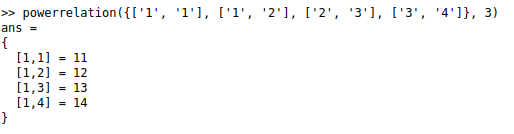
\includegraphics[scale=0.60]{/home/adrian/Imágenes/Capturas de pantalla/Captura desde 2022-10-08 17-39-59.png}
\label{}
\end{figure}
\newpage
\section*{Ejercicio 2}
Within the folder “files”, find a TEX file in whose content appears the string \textbackslash
usepackage\{amsthm, amsmath\}. Note: use grep and escape the special
characters with \textbackslash. Complete the proof and answer the question.
\begin{figure}[htp]
\centering
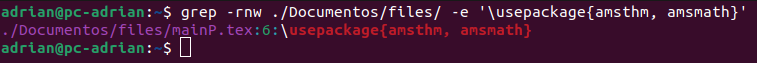
\includegraphics[scale=0.60]{/home/adrian/Imágenes/Capturas de pantalla/Captura desde 2022-10-08 19-22-32.png}
\label{}
\end{figure}
\\
El archvo a se llama mainP.tex. En él se encuentra la resolución del segundo ejercicio.
\end{document}

